\documentclass{sig-alt-release2}
\usepackage{url}
\usepackage{color}
\usepackage{graphics,graphicx}

\usepackage{epsfig}
\usepackage{epstopdf}

\usepackage{colortbl}
\usepackage{multirow}
\usepackage{booktabs}
\usepackage{ifthen}

\begin{document}

\newcommand{\todo}[1]{\textcolor{red}{#1}}
\def\newblock{\hskip .11em plus .33em minus .07em}

\conferenceinfo{DIM3} {2010, Glasgow, UK}
\CopyrightYear{2011}
\clubpenalty=10000
\widowpenalty=10000

\title{Meow - Design and Specification Report}

\numberofauthors{4}
\author{
\alignauthor
    \affaddr{Team G}\\
    \affaddr{DIM3}\\
    \affaddr{Ewan Baird 0806543B@student.gla.ac.uk\\
             Heather Hoaglund-Biron 1003914H@student.gla.ac.uk\\
             Gordon Martin 0800902M@student.gla.ac.uk\\
             James McMinn 0800890M@student.gla.ac.uk}
}
\maketitle

\begin{abstract}
This document details the design and specification of the ``Meow'' web application for Team G, a Twitter- and Tumblr-like site where people can share text, images, and more in a live stream of messages.
\end{abstract}

\section{Aim of Application}
The application is an online micro blogging website which allows users to post messages with embedded multimedia content, and to view a real time stream of messages from other users.

We aim to learn what the process of creating a web app involves, while learning how to use technologies like Django.

%Describe this shit
\begin{itemize}
\item	Required Functionality:

Registration

Log in/out

RSS feed

Real time Message Stream

Post Messages

\item	Desired Functionality:

Followers/Following

@ Messages (Mentions)

Time Stamps

URL parsing

Display Pictures

Profile Page

Search (Users and Messages)

Hash tags

Mobile browser support
\end{itemize}

We plan to achieve all of the required functionality as well as a fair amount of the desired functionality. We are making the application slightly more complex than the problem description entails, but we believe we can achieve this, and it will give our project an edge over other similar ones. It is designed to be distributed across the web.

%Describe each component
\section{Application Architecture}

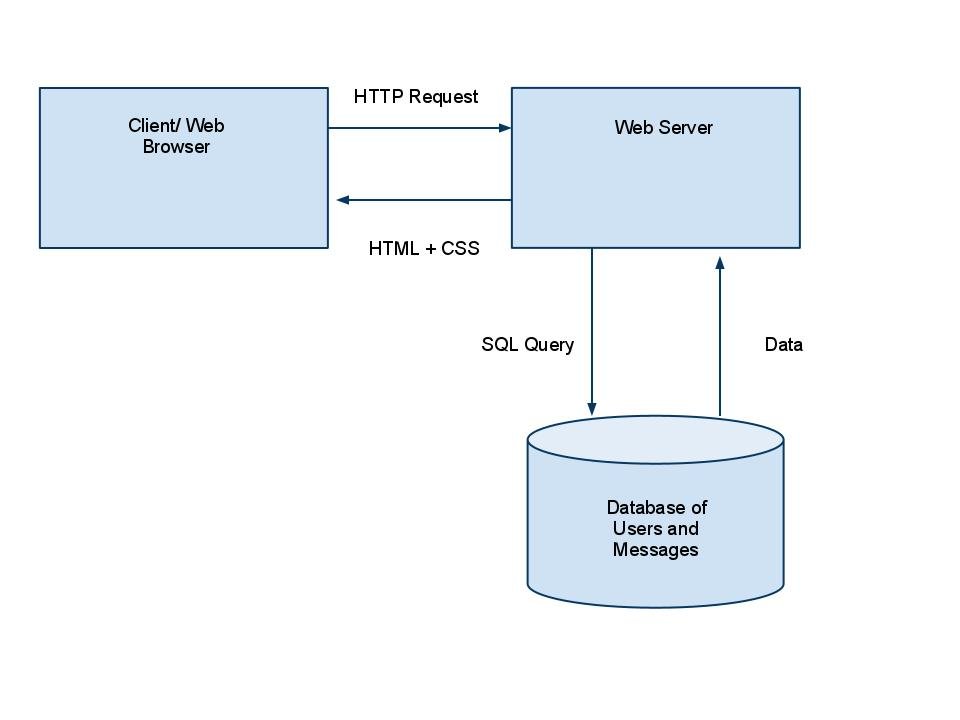
\includegraphics[width=250px]{images/architecture.jpg}

%Describe each entity, fix Metion to Mention, VARCHAR max lengths.
\subsection{ER Diagram}

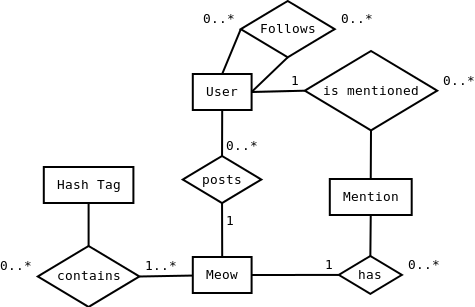
\includegraphics[width=250px]{images/erdiagram.png}

Our team has used a range of technologies to split the project into different sub-systems. For instance, Django abstracts the concern of micro-managing the creation and querying of a database from our team, so that we may concentrate on the functionality and design of the web application. Furthermore, Django manages the back end of the website. 

We have abstracted the concern of scripting (which will `carry' the functionality of the website) from the design. The scripting of the website will be implemented using JavaScript, and the design handled by HTML and CSS.

Using Django allows us to focus on building the application and avoid the tedious boiler plate that normally goes with building an application. This allows us to rapidly build the application and focus on functionality without wasting time on the more tedious aspects of application development.

Another advantage of a web application framework is structuring and organisation. Django provides us with a fixed structure to adhere to. This is especially important in a team project, as each member should implicitly know where to code.

A number of other web application frameworks are available such as Ruby On Rails, CakePHP and Pylons. We chose to implement Meow using Django as it is the framework we have the most experience using.

Using Django has some disadvantages.  For example, we are now restricted to using the MVT architecture used by Django. We are also more vulnerable as we rely on the Django developers for security and other updates. 

\section{Message Parsing}

\begin{verbatim}
JSON message examples to represent 
	user posts to the system.
[
	{"uid":  	26,
	"mid":  	10245674,
    "username": "Sam",
    "time": 	1297516219,
    "message":  "why do i get to pick how thick cut my 
				marmalade is, but I have no choice with
				jam!? #mundanepoint",
	"media":	{"type": "image", "URL":
			"http://marmaladecentral.org/mediumcut.jpg"}
	},
	{"uid":  	57,
	"mid":  	10245674,
    "username": "Bob",
    "time": 	1297516201,
    "message":  "Egyptians complain soooo much, doubt
		they have as many speed cameras as us! #topical"
	"media":	{"type": "video", "URL":
			"http://www.youtube.com/watch?v=mJ1qvlUktBE"}
	}
]  
\end{verbatim}

As JSON is designed to be as human readable as possible, the messages are not complicated. They are comprised of the user ID to represent the user which posted the message and the display name of that user. The time is stored as the Unix Epoch (i.e. the number of seconds since 1st January 1970). The text content of the message and any hash tags are stored in the ``message'' field. The ``media'' field contains both the type of media (image, video, music, text or none) and the URL for the embedded content. If the media type is ``none'' then the URL will be nulled. This simple format should include all the necessary components of a users message.


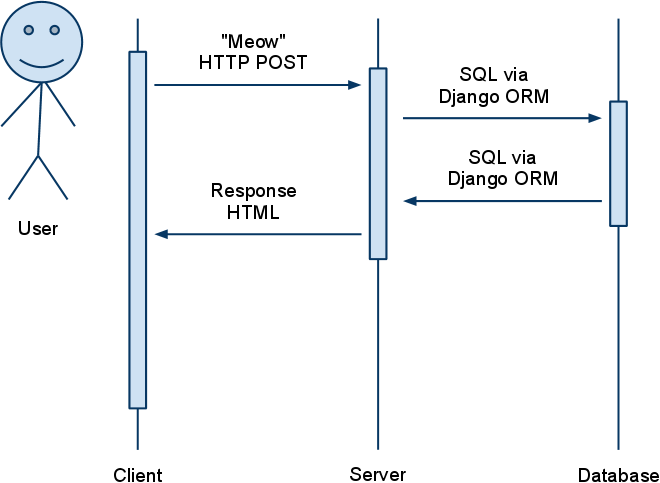
\includegraphics[width=250px]{images/sequence.png}

\section{Client Interface}

\subsection{Wireframe}

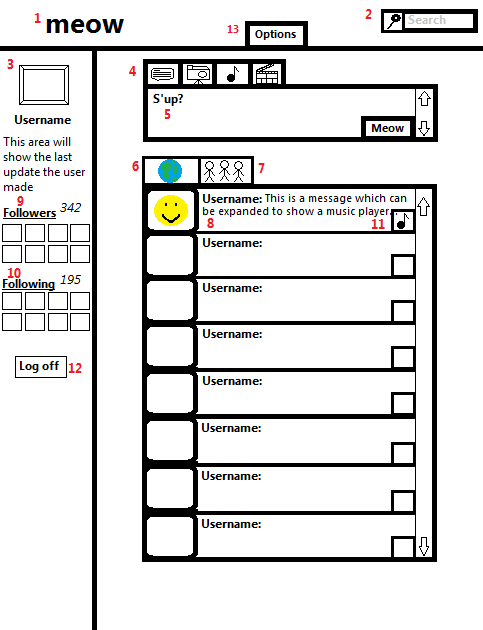
\includegraphics[width=250px]{images/wireframe.png}

\begin{enumerate}

\item Logo: This will act as a hyperlink returning the user to the home page (In this case it takes the user to this page).

\item Search Function: This allows users to search for other users, or message content through hash tags. Messages can be filtered by their content tag (11) type. Changing the search options is achieved through a drop down menu accessed by clicking the magnifying glass.

\item Display Picture: A small image stored on the server used to represent the user. This image can be changed through the options page.

\item Content Type: An optional tag attached to each post, which allows the user to specify what is contained in the message. A content type is not required.

\begin{itemize}
\item Text - This allows the user to post larger messages
\item Image - Allows the user to embed an image file from a URL
\item Music - Allows the user to embed a music clip through a player
\item Video - Allows the user to embed a video file into the message
\end{itemize}

\item Message Input Box: This is the area where the user inputs the content of a message then posts it to the Stream. The Enter Key or the ``Meow'' button are used to submit.

\item Global Stream button: This button displays the messages from every user on the system in the stream.

\item `Following' Stream button: This button displays the messages from users which the user is currently following, and themselves.

\item Stream Message: Comprised of a display picture, user name, content tag and text. Messages can be expanded out if they have content tag (11). The User name acts as a hyperlink to their profile page.

\item Followers: This section shows 8 random people who have opted to follow the user. The 8 display pictures act as links to the respective profiles. The word `Followers' is a hyperlink which takes the user to a page to manage followers and people following (10). The number indicates how many people are following the user.

\item Following: This section shows 8 random people who are being followed by the user. The 8 display pictures act as links to the respective profiles. The word `Following' is a hyperlink which takes the user to a page to manage followers(9) and people following. The number indicates how many people the user is following.

\item Content tag: This indicates the type of content contained within the expanded message, if available (otherwise blank).

\item Log off: This returns the user to the log in page.

\item Options: This takes the user to the options page which allows them to edit their profile details.

\end{enumerate}

\subsection{Use Case Descriptions}

This section details 4 key use cases for the system.

\begin{enumerate}

\item Login - On visiting the site, the user will be prompted to log in to access the rest of the site content. This provides a basic level of security and allows users to access their personal profile.

\item Post Message - On the home page which is reached after logging in, the user is able to post messages. This is done by entering text into the text box and pressing the ``Meow'' button or pressing the `Enter' key. Users can assign media content to their message by clicking one of the content buttons, which brings up a prompt to embed a URL link.

\item Follow User - Following a user makes all posts by that user appear in the ``following stream''. The first stage of following a user is reaching their profile page, which can be done in various ways: Users can press a user name on the global stream, search for a user name, directly type in the URL or if that user is following them, click the name from the `followers/following' page. On the profile page of another user, pressing the `Follow' button adds the user to the list of users being followed. If a user is being followed already, the `Follow' button becomes `Unfollow'.

\item Search - A lower priority, but still desired functionality, is the ability to search. Users will be able to go to the search bar at the top of the page and search for words in the message stream, which will then make the related messages appear below. Presumably they will also be able to search for other users in the same way.

\end{enumerate}

\section{Design Decisions}

The message streams are the most important components which will require dynamic updating. As a new message is posted to the service, other users currently using the service will be notified using AJAX and the jQuery JavaScript framework, with the newly posted messages being sent to the client in JSON format.

One of the key design goals for Meow was to develop a clean and simple website. Users should be instantly familiar with the mechanics of the website if they have used Twitter, Tumbler or any other similar application, and if not, should still be able to understand the site in a short amount of time.

%This needs changed, purple is no more...
The colour scheme will feature a sedate purple motif which will hopefully be inoffensive and visually appealing.

\section{Summary and Future Work}

Our application combines the ideas of Twitter and Tumblr into a multimedia message streaming web application. To create it, we plan to combine the use of Django, XHTML, CSS, JavaScript, and SQL.

The next stage of development is implementation. We have a simple layout already implemented featuring borders and a main header, however, functionality is yet to be added.

\section{Acknowledgements}

%Do we need this?

\bibliographystyle{abbrv}
\bibliography{sig-proc}
%References, Django, AJAX, JSON, JQuery, any others.

\end{document}
